\section{Blockchain Infix proofs}

\subsection{Construction}

While the previous proofs we constructed were proving predicates on the blocks
and transactions pertaining to the chain suffix of the last $k$ blocks, similar
to the kind of proofs possible with \cite{KLS}, we note that the most useful
class of proofs would allow proving more general predicates that can depend on
multiple blocks, sometimes even blocks buried deep within the blockchain.

We will now extend our prover to support this generalization of predicates. The
generalized prover allows proving any predicate $Q(\chain)$ that depends on a
number of blocks that can appear anywhere within the chain. These blocks
constitute a \textit{subchain} $\chain'$ which is a subsequence of the original
blockchain. For our proofs to work, the blocks contained within the subchain
have to be $k$-stable; that is, they cannot be one of the most recent $k$
blocks.

The proofs are able to prove any predicate of the general class of predicates
that depend on both the inclusion of the blocks of the subchain as well as
their relative order within the subchain. This allows proving powerful
statements such as, for example, whether a transaction took place at any point
in history, or even ``following the money'' and proving a claim that a certain
coin was moved between a series of addresses in a particular order.

The manner to construct these proofs is shown in
Algorithm~\ref{alg.nipopow-infix-prover}. The infix prover accepts two
parameters: The chain $\chain$ which is the full blockchain and $\chain'$ which
is a subchain of the blockchain whose blocks are of interest for the predicate
in question. This prover simply calls the previous suffix prover to produce a
proof as usual. Then, having the prefix $\pi$ and suffix $\chi$ of the suffix
proof in hand, the infix prover adds a few auxiliary blocks to the prefix
$\pi$. The prover ensures that these auxiliary blocks form a verifiable chain
with the rest of the proof $\pi$ in a manner that the blocks can be arranged in
topological order such that a pointer exists from each non-Genesis block to a
preceeding block and each preceeding block is pointed to by a unique block.
Such auxiliary blocks are collected as follows: For every block $B$ of the
subchain $\chain'$, the immediate previous ($E'$) and next ($E$) blocks in the
proof $\pi$ are found. Then, a chain of blocks $R$ which connects $E$ back to
$B'$ is found by the algorithm followDown. Finally, observe that if $E'$ is of
level $\mu$, then there can be no other $\mu$ level superblock between $E'$ and
$B'$, otherwise it would have been included in $\pi$. Therefore, block $B'$
already contains a pointer to $E'$ in its interlink, completing the chain.

\import{./}{algorithms/alg.nipopow-infix-follow.tex}

The way to connect a superblock to a previous lower-level block is implemented
in Algorithm~\ref{alg.nipopow-infix-prover} as the followDown algorithm. Notice
that block $B'$ cannot be of higher or equal level than block $E$, otherwise it
would be equal to $E$ and the followDown algorithm would return immediately.
The algorithm then proceeds as follows: Starting at block $E$ which here is
marked as $hi$, it tries to follow a pointer to as far as possible. If
following the pointer surpasses block $B'$, which here is marked as $lo$, then
the following is aborted and a lower level is tried, which will cause a smaller
step within the skiplist. If a pointer was followed without surpassing $B'$,
the operation continues from the new block, until eventually $B'$ will be
reached, which concludes the algorithm.

\import{./}{algorithms/alg.nipopow-infix-prover.tex}

An example of the kind of auxiliary sequences that followDown produces is seen
in Figure~\ref{fig.infix}. This is only a portion of the proof shown at the
point where the superblock levels are at level $4$, but a descend to level $0$
was necessary so that a regular block would be included in the chain. Note that
the level $0$ block can jump immediately back up to level $4$ because it has a
high-level pointer.

\begin{figure}[h]
    \caption{An infix proof descending down to level $0$ and back up to level
    $4$. Only blue blocks are included in the proof. Blue blocks of level $4$
    are part of $\pi$, while the blue blocks of level $1$ and $3$ are produced
    by followDown to get to the block of level $0$ which is part of $\chain'$.
    Notice how in this proof the blocks happened to be distributed slightly
    different from expectation and there are two consecutive $0$-level blocks.}
    \centering
    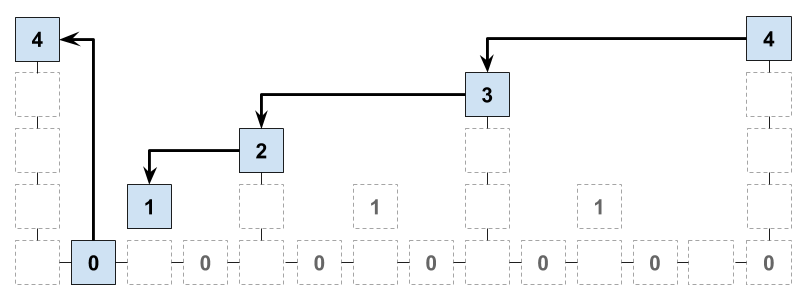
\includegraphics[width=\columnwidth,keepaspectratio]{figures/infix.png}
    \label{fig.infix}
\end{figure}

\subsection{Security}
The security of infix proofs follows immediately from
Theorem~\ref{thm.security}. To see this, notice that the verifier will still
verify the suffix proof. Upon determining which of the blockchains is the
longest securely, it will subsequently verify that the subchain blocks have
been properly included within the referenced chain. However, if the chain is
honest, this proof of inclusion cannot be produced by the adversary.

\subsection{Succinctness}
As long as the number of blocks on which the predicate depends is
polylogarithmic with respect to the chain length, our proofs remain succinct.
Specifically, the proof size for the suffix has exactly the same size. Then
the part of the proof that is of interest is the output of the followDown
algorithm. However, notice that this algorithm will on average produce as many
blocks as the difference of levels between $B'$ and $E$, which is at most
logarithmic in the chain size. Hence the proof sizes will be in expectation
$(m + |\chain'|)\log(|\chain|)$, which remains succinct if $|\chain'| \in
O(polylog(|\chain|))$.
